\documentclass[manuscript]{stjour}

\journalname{Open Mind}

%%%%%%%%%%%%%%%%%%%%%%%%%%%%%%%%%%%%%%%%%%%%%%%%%%
%% For production only, not authors:
%%\documentclass[OpenMind,finalfonts]{stjour}

%%%%%%%%%%% Please supply information %%%%%%%%%%%%%%%%%%%%%%%%%

\supplementslinks{Links to Supplementary Materials.}


%%%%%%%%%%% to be supplied by MIT Press, only %%%%%%%%%%%%%%%%%

\citation{CITATION}

\received{RECEIVED}
\accepted{ACCEPTED}
\published{PUBLISHED}

%% DOI address:
\setdoi{DOI}

%%%%%%%% End MIT Press commands %%%%%%%%%%

%%%%%%%%%%%%%%%%%%%%%%%%%%%%%%%%%%%%%%%%%%%%%%%%%%%%%%%%%%%%%%%
%% author definitions should be placed here:

\usepackage{booktabs}
\usepackage{listings}
\lstset{literate={~} {$\sim$}{1}}
\lstset{basicstyle=\ttfamily}

\begin{document}

\title[Word learning consistency and variability]{Consistency and variability in children's word learning across languages}

\author[Braginsky, Yurovsky, Marchman, Frank]{
      Mika Braginsky\affil{1},
      Daniel Yurovsky\affil{2},
      Virginia A. Marchman\affil{3},
      and Michael C. Frank\affil{3}}

  \affiliation{1}{Department of Brain and Cognitive Sciences, Massachusetts Institute of
Technology}
  \affiliation{2}{Department of Psychology, University of Chicago}
  \affiliation{3}{Department of Psychology, Stanford University}

\correspondingauthor{Mika Braginsky}{mikabr@mit.edu}

\keywords{ word learning,  language acquisition,  corpus analysis}

\begin{abstract}
Why do children learn some words earlier than others? The order in which
words are acquired can provide clues about the mechanisms of word
learning. In a large-scale corpus analysis, we use parent-report data
from over 32,000 children to estimate the acquisition trajectories of
around 400 words in each of 10 languages, predicting them on the basis
of independently-derived properties of the words' linguistic environment
(from corpora) and meaning (from adult judgments). We examine the
consistency and variability of these predictors across languages, by
lexical category, and over development. The patterning of predictors
across languages is quite similar, suggesting similar processes in
operation. In contrast, the patterning of predictors across different
lexical categories is distinct, in line with theories that posit
different factors at play in the acquisition of content words and
function words. By leveraging data at a significantly larger scale than
previous work, our analyses identify candidate generalizations about the
processes underlying word learning across languages.
\end{abstract}

\section{Introduction}

Despite tremendous individual variation in children's rate of
development \citep{fenson2007}, the first words that they utter are
strikingly consistent \citep{tardif2008,schneider2015}: they tend to
talk about important people in their life (``mom'', ``dad''), social
routines (``hi'', ``uh-oh''), animals (``dog'', ``duck''), and foods
(``milk'', ``banana''). Even as children learn from their own
experiences and according to their own interests
\citep{mayor2014,nelson1973}, their vocabulary grows rapidly, typically
adding more nouns, but also verbs (``go'') and other predicates
(``hot'') to their repertoires. Over just their first three years,
children learn hundreds, even thousands of words
\citep{fenson1994,mayor2011}.

One classic approach to word learning focuses on the specific mechanisms
that children bring to bear on the learning problem. For example, across
many laboratory experiments, a variety of mechanisms have been
identified as plausible drivers of early word learning, including
co-occurrence based and cross-situational word learning
\citep{schwartz1983,yu2007}; social cue use \citep{baldwin1993}; and
syntactic bootstrapping \citep{gleitman1990,mintz2003}. The ability to
identify which of these mechanisms is most explanatory has been
challenging. Indeed, many theories of early word learning take
multiplicity of cue types and mechanisms as a central feature (e.g.,
\citealp{hollich2000,bloom2000}). As important as this work is, though,
these studies typically are aimed at understanding how one or a small
handful of words are learned in the laboratory under precisely-defined
learning conditions. They do not directly address questions regarding
the developmental composition and ordering of growth in the lexicon
across many different children in their natural environments, nor
whether these patterns are consistent across different languages.

An alternate approach to early word learning asks why some words are
learned so early and some much later. This question about the order of
the acquisition of first words can provide a different window into the
nature of children's language learning. Posed as a statistical problem,
the challenge is to find what set of variables best predicts the age at
which different words are acquired. Previous work using this approach
has revealed that, in English, within a lexical category (e.g., nouns,
verbs), words that are more frequent in speech to children are likely to
be learned earlier \citep{goodman2008}. Further studies have found
evidence that a variety of other semantic and linguistic factors are
related to word acquisition, such as salience and iconicity
\citep{hills2009,stokes2010,perry2015,roy2015,swingley2017}.

But these exciting findings are limited in their generality because each
study used a different dataset and focused on different predictors. In
addition, nearly all studies to date have exclusively analyzed data from
English-learning children, providing no opportunity for cross-linguistic
comparison of the relative importance of the many relevant factors under
consideration. Cross-linguistic comparisons are critical to identifying
the universal mechanisms that are in play for all children and
differentiating them from patterns of acquisition that emerge due to the
particulars of a given language or culture \citep{slobin1985,bates1987}.
Our goal here is to extend these classic approaches by assessing the
degree to which the predictors of word learning are consistent across
different languages, as well as whether there are similar patterns
across different lexical categories.

The primary tool for characterizing the breadth of children's early
vocabularies in these previous studies has been structured parent
report. Naturalistic language samples and experimental methods are both
valuable methods for assessing aspects of child language
\citep{bornstein1998,fernald2006}. But outside of a few ultra-dense
transcripts (e.g., \citealp{roy2015}), neither method typically provides
the kind of holistic and comprehensive view that comes from parent
report. We focus in particular on the MacArthur-Bates Communicative
Development Inventory (CDI; \citealp{fenson2007}), a family of
parent-report vocabulary checklists in which parents are asked whether
their child ``understands'' or ``understands and says'' a large set of
individual words.

The CDIs are an inexpensive and widely-used method for gathering
reliable and valid data about the nature and extent of young children's
productive and receptive vocabularies (see \citealp{fenson1994} for
review; cf. \citealp{feldman2000, fenson2000}). Although CDIs cannot
exhaustively capture all words in a child's vocabulary
\citep{mayor2011}, they do give an estimate of a child's knowledge about
several hundred words, far more than the handful that are typically
tested in a lab experiment. CDI estimates of vocabulary size are highly
correlated with children's overall vocabulary knowledge as assessed with
naturalistic observation or using standardized tests \citep{fenson2007}.
Of course, any parent report measure is subject to reporting biases. The
CDIs were designed to minimize these by asking parents to report only on
observable behaviors that are currently (rather than retrospectively)
demonstrated and to identify words from a pre-selected list (rather than
having them recall them on their own).

Because of the low cost of administering CDI instruments, it is
relatively easy to gather samples containing data about hundreds or
thousands of children. Such large samples in turn make it possible to
recover stable estimates of the average difficulty of individual words,
even if individual children's data may be noisy. Thus, CDI data are
typically the dataset of choice for the studies of vocabulary
composition described above.

Finally, CDI instruments have been adapted in dozens of different
languages, providing an opportunity for cross-linguistic comparison. The
American English CDI is not simply translated to other languages
verbatim; instead, expert groups of researchers adapt the form for their
particular linguistic and cultural situation. This process leads to a
wide range of forms that share a common structure, but contain sets of
words that are customized to a particular language and culture. Thus,
cross-linguistic comparisons do not reflect children's acquisition of a
single set of words, but instead capture relevant information regarding
patterns of children's vocabulary development using instruments designed
specifically for each language.\footnote{Of course, observational data
  of this type are still open to other sources of bias, a point we
  return to in the Discussion.}

In our study, we conduct cross-linguistic comparisons of the acquisition
trajectories of children's early-learned words using Wordbank
(\href{http://wordbank.stanford.edu}{wordbank.stanford.edu};
\citealp{frank2016}), an open repository that aggregates administrations
of the CDI across languages. We integrate these acquisition trajectory
data with independently-derived characterizations of the word learning
environment from other datasets. The use of secondary datasets is
warranted because no currently available resource provides data on both
children's language environments and their learning outcomes for more
than a small handful of children. In particular, we derive our estimates
of the language environment from transcripts of speech to children in
the CHILDES database \citep{macwhinney2000} and measures of
meaning-related word properties from available psycholinguistic
databases. This data-integration methodology was originated by
\citet{goodman2008}; it relies on large samples to average out the
(substantial) differences among children and care environments. While
introducing additional sources of variability, this approach allows for
analyses that cannot be performed on smaller datasets that measure only
children or environments but not both.

To measure environmental input, we used existing adult speech data from
the CHILDES database to estimate each word's frequency (a) in speech to
children, (b) as a sole utterance constituent, (c) in utterance-final
position, and the (d) mean length of utterances (MLU) containing that
word. While crude, these measures are both easy to compute and
relatively comparable across languages. To derive proxies for the
meaning-based properties of each word, we accessed available
psycholinguistic norms using adult ratings of each word's (a)
concreteness, (b) valence, (c) arousal, and (d) association with babies.
Integrating these estimates, we predict each word's acquisition
trajectory, assessing the relative contributions of each predictor, how
predictors change over development, and how predictors differ by lexical
category. Since vocabulary composition differs in comprehension and
production (e.g., \citealp{benedict1979}), we conduct our analyses
independently on each.

These analyses address two questions. First, we ask about the degree of
consistency across languages in the relative importance of each
predictor. To do so, we compare the estimates for the effect of each
predictor for each language and conduct analyses that determine the
likelihood that the consistency of the estimates did not occur by
chance. Consistency in the patterning of predictors would suggest that
similar information sources are important for learners, regardless of
language, and that linguistic dissimilarities (e.g., greater
morphological complexity in Russian, greater phonological complexity in
Danish) do not dramatically alter the course of acquisition. Conversely,
evidence for variability across languages would show the degree to which
learners face different challenges in learning different languages,
posing a challenge for more universalist accounts. Further,
systematicity in the variability between languages would reveal which
languages are more similar than others in the structure of these
different challenges.

Second, we ask which lexical categories are most influenced by
linguistic environment factors, like frequency and utterance length,
compared with meaning-based factors like concreteness and valence.
Division of dominance theory suggests that nouns might be more sensitive
to meaning factors, while predicates and closed-class words might be
more sensitive to linguistic environment factors \citep{gentner2001}.
And on syntactic bootstrapping theories \citep{gleitman1990}, nouns are
argued to be learned via frequent co-occurrence (operationalized by
frequency) while verbs might be more sensitive to syntactic factors
(operationalized here by utterance length; \citep{snedeker2007}). Thus,
examining the relative contribution of different predictors across
lexical categories can help test the predictions of influential theories
of acquisition.

\section{Methods}

The code and data for these analyses are available at
\href{https://github.com/mikabr/aoa-prediction}{github.com/mikabr/aoa-prediction}.

\subsection{Acquisition trajectories}

To estimate the trajectory of words' acquisition, we used vocabulary
data collected using CDI instruments adapted in many different
languages, including both Words \& Gestures (WG) and Words \& Sentences
(WS) forms. When filling out a CDI form, parents are either asked to
indicate whether their child ``understands'' (comprehension) or
``understands and says'' (production) each of around 400-700 words. Both
comprehension and production are queried for younger children and only
production is queried for older children. We included data from the
items on the WG form for comprehension, and data from the items in
common between the WG and WS forms for production. Placeholder items,
such as ``child's own name,'' were excluded. Table~\ref{tab:langstats}
gives an overview of our acquisition data
(\citealp{kovacevic1996,bleses2008,boudreault2007,trudeau2011,caselli2012,caselli1995,simonsen2014,vershinina2011,yeliseyeva2009,fenson2003,eriksson2002,acarlar2008};
also see Supplemental Information Figure~SI.1 for the age distributions). Each
of the datasets were collected in the language of the community, e.g.,
the Mexican Spanish CDI data were collected in several areas of Mexico;
longitudinal administrations were excluded.

\begin{table}[t]

\caption{\label{tab:langstats}Statistics for data from Wordbank and CHILDES. N indicates number of children.}
\centering
\begin{tabular}{>{\bfseries}lrrlrlrr}
\toprule
\multicolumn{1}{c}{} & \multicolumn{1}{c}{} & \multicolumn{2}{c}{Production} & \multicolumn{2}{c}{Comprehension} & \multicolumn{2}{c}{CHILDES} \\
\cmidrule(l{3pt}r{3pt}){3-4} \cmidrule(l{3pt}r{3pt}){5-6} \cmidrule(l{3pt}r{3pt}){7-8}
Language & CDI items & N & Ages & N & Ages & Types & Tokens\\
\midrule
Croatian & 388 & 627 & 8-30 & 250 & 8-16 & 12,064 & 218,775\\
Danish & 381 & 6,112 & 8-36 & 2,398 & 8-20 & 4,956 & 195,658\\
English (American) & 393 & 7,312 & 8-30 & 1,792 & 8-18 & 45,597 & 7,679,042\\
French (Quebec) & 396 & 1,364 & 8-30 & 537 & 8-16 & 28,819 & 2,551,113\\
Italian & 392 & 1,400 & 7-36 & 648 & 7-24 & 7,544 & 188,879\\
Norwegian & 380 & 7,466 & 8-36 & 2,374 & 8-20 & 10,670 & 231,763\\
Russian & 410 & 1,805 & 8-36 & 768 & 8-18 & 5,191 & 32,398\\
Spanish (Mexican) & 399 & 1,891 & 8-30 & 788 & 8-18 & 33,529 & 1,609,614\\
Swedish & 371 & 1,367 & 8-28 & 467 & 8-16 & 8,815 & 359,155\\
Turkish & 395 & 3,537 & 8-36 & 1,115 & 8-16 & 6,503 & 44,347\\
\bottomrule
\end{tabular}
\end{table}

For each word, the CDI data yield a trajectory reflecting the number of
children that are reported to understand or produce the word at each age
covered by the instrument (see Figure~\ref{fig:demotraj} for some
examples).

\begin{figure}

{\centering 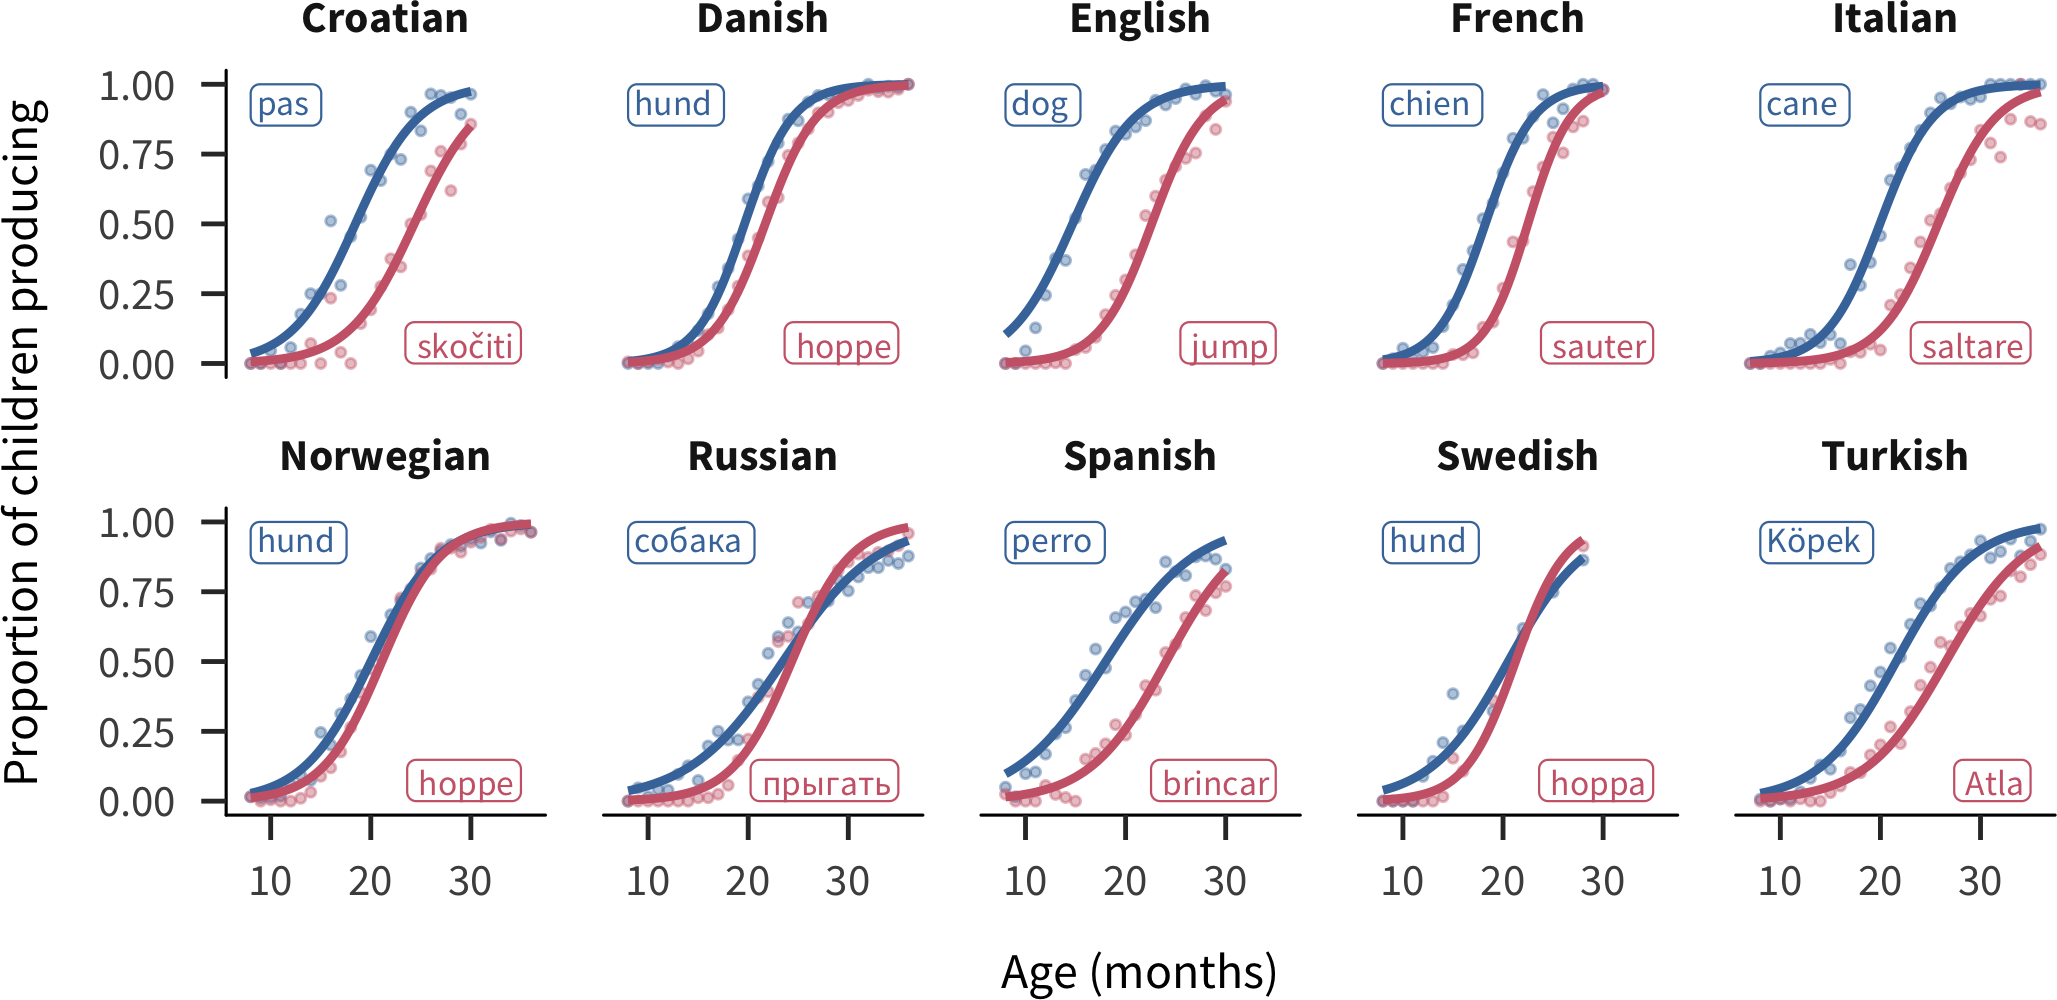
\includegraphics[width=\textwidth]{demotraj-1}

}

\caption{Example production trajectories for the words "dog" and "jump" across languages. Points show the proportion of children producing each word for each one-month age group. Lines show the best-fitting logistic curve. Labels show the forms of the words in each language.}\label{fig:demotraj}
\end{figure}

\subsection{Word properties}

\subsubsection{Overview}

For each word in each of our 10 languages, we used corpora of
child-directed speech in that language from CHILDES to obtain an
estimate of its frequency, the mean length of utterances in which it
appears, its frequency as the sole constituent of utterance, and its
frequency in utterance final position. We also computed each word's
length in phonemes.

In addition, each word's concreteness, valence, arousal, and relatedness
to babies\footnote{Previous studies have shown robust consistency in the
  types of words that children learn very early \citep{tardif2008}.
  These words seem to describe concepts that are important or exciting
  in the lives of infants in a way that standard psycholinguistic
  features like concreteness do not. Capturing this intuition
  quantitatively is difficult, but \citet{perry2015} provides a proxy
  measure as a first step. This measure is simply the degree to which a
  particular word was ``associated with babies''. Intuitively, we expect
  this measure to capture the degree to which words like ``ball'' or
  ``bottle'' feature heavily in the environment (and presumably, mental
  life) of many babies.} were compiled from ratings based on previous
studies using adult raters. Since existing ratings are primarily
available for English, we mapped all words onto translation equivalents
across CDI forms, verified by native speaker judgement, allowing us to
use the English ratings across languages. Of the resulting translation
equivalent meanings, 35\% occur only in one language, 51\% occur in more
than one but not all languages, and 14\% occur in all languages. While
necessarily imperfect, this method allows us to examine languages for
which limited resources exist. Example words for these predictors in
English are shown in Table~\ref{tab:extremes} (also see
Figures~SI.2 and SI.3 for the distributions of values of each predictor).

\begin{table}[t]

\caption{\label{tab:extremes}Items with the highest and lowest values for each predictor in English.}
\centering
\resizebox{\linewidth}{!}{
\begin{tabular}{lll}
\toprule
Predictor & Highest & Lowest\\
\midrule
Arousal & naughty, money, scared & today, asleep, shh\\
Babiness & baby, bib, bottle & jeans, penny, donkey\\
Concreteness & apple, baby, ball & that, now, how\\
Final frequency & book, it, there & put, when, give\\
Frequency & you, it, that & babysitter, rocking chair, grrr\\
MLU & daddy, when, day & ouch, thank you, peekaboo\\
Number phonemes & refrigerator, cockadoodledoo, babysitter & i, eye, ear\\
Solo frequency & no, yes, thank you & feed, bathroom, tooth\\
Valence & happy, hug, love & ouch, hurt, sick\\
\bottomrule
\end{tabular}}
\end{table}

Each numeric predictor was centered and scaled (within language) so that
all predictors would have comparable units.

\subsubsection{Frequency}

For each language, we derived unigram counts based on all corpora in
CHILDES for that language. Frequencies varied widely both within and
across lexical categories (see Figure~SI.4). Each
word's count was summed across inflected forms (e.g., ``dogs'' counts as
``dog'') and synonyms (e.g., ``father'' counts as ``daddy''). For
polysemous words (e.g., ``orange'' as in color or fruit), occurrences
were split uniformly between the senses on the CDI (there were only
between 1 and 10 such word pairs in the various languages; in the
absence of cross-linguistic corpus resources for sense disambiguation,
this is a necessary simplification). Counts were normalized to the
length of each corpus, Laplace smoothed (i.e., counts of 0 were replaced
with counts of 1), and log transformed.

\subsubsection{Solo and Final Frequencies}

Using the same dataset as for frequency, we estimated the frequency with
which each word occurred as the sole word in an utterance, and the final
word of an utterance (not counting single-word utterances). Solo and
final counts were normalized to the length of each corpus, Laplace
smoothed, and log transformed. Since both of these estimates are by
necessity highly correlated with frequency, we then residualized unigram
frequency out of both, so that values reflect an estimate of the effects
of solo frequency and final frequency over and above frequency.

\subsubsection{MLU}

MLU is only a rough proxy for syntactic complexity, but is relatively
straightforward to compute across languages (in contrast to other
metrics). For each language, we estimated each word's MLU by calculating
the mean length in words of the utterances in which that word appeared,
for all corpora for that language. For words that occurred fewer than 10
times, MLU estimates were treated as missing.

\subsubsection{Number of phonemes}

In the absence of consistent resources for cross-linguistic
pronunciation, we computed the number of phonemes in each word in each
language based on phonemic transcriptions of each word obtained using
the eSpeak tool \citep{duddington2012}. We then spot-checked these
transcriptions for accuracy.

\subsubsection{Concreteness}

We used previously collected norms for concreteness
\citep{brysbaert2014}, which were gathered by asking adult participants
to rate how concrete the meaning of each word is on a 5-point scale from
abstract to concrete.

\subsubsection{Valence and Arousal}

We also used previously collected norms for valence and arousal
\citep{warriner2013}, for which adult participants were asked to rate
words on a 1-9 happy-unhappy scale (valence) and 1-9 excited-calm scale
(arousal).

\subsubsection{Babiness}

We used previously collected norms of ``babiness'', a measure of
association with infancy \citep{perry2015} for which adult participants
were asked to judge a word's association with babies on a 1-10 scale.

\subsubsection{Lexical category}

Category was determined on the basis of the conceptual categories
presented on the CDI form (e.g., ``Animals'', ``Action Words''), such
that the Nouns category contains common nouns, Predicates contains
verbs, adjectives, and adverbs, Function Words contains closed-class
words (following \citealp{bates1994}), and the remaining items are
binned as Other.

\subsubsection{Imputation}

The resulting set of predictor value for each language had varying
numbers of missing values, depending on resource availability (number
phonemes 0\%, concreteness 0\%-1\%, arousal and valence 8\%-13\%,
{[}solo/final{]} frequency 2\%-14\%, babiness 10\%-33\%, MLU 2\%-53\%).
We used iterative regression imputation to fill in these missing values
by first replacing missing values with samples drawn randomly with
replacement from the observed values, and then iteratively imputing
values for a predictor based on a linear regression fitting that
predictor from all others.

\subsubsection{Collinearity}

A potential concern for comparing coefficient estimates is predictor
collinearity. Fortunately, in every language, the only relatively high
correlations were between MLU and solo frequency (mean over languages
\(r = -0.44\)), as expected given the similarity of these factors, along
with modest correlations between frequency and concreteness (mean over
languages \(r = -0.36\)) and between frequency and number of phonemes
(mean over languages \(r = -0.33\)), a reflection of Zipf's Law
\citep{zipf1935}. More importantly, the variance inflation factor for
each predictor in each language was no greater than 2.27, indicating
that multicollinearity among the predictors is low (see
Figure~SI.5 for the full set of pairwise
correlations and Figure~SI.6 for the variance inflation
factors).

\subsection{Analysis}

We used mixed-effects logistic regression models (fit with the
MixedModels package in Julia; \citealp{bates2018}) to predict whether
each child understands/produces each word from the child's age,
properties of the word, interactions between each property and age, and
interactions between each property and lexical category (which was
contrast coded). Each model was fit to all data from a particular
language and included a random intercept for each word and a random
slope of age for each word. Computational and technical limitations
prevented us from including random effects for child or including data
from all languages in one joint model.

The magnitude of the standardized coefficient on each property gives an
estimate of its independent contribution to words being
understood/produced by more children. Interactions between properties
and age give estimates of how this effect is modulated for
earlier-learned and later-learned words. For example, a positive effect
of babiness means that words associated with babies are learned earlier;
a negative interaction with age means that high babiness primarily leads
to higher rates of production and comprehension for younger children.
Similarly, interactions between properties and lexical category give
estimates of how the effect differs among nouns, predicates, and
function words.

\section{Results}

\begin{figure}

{\centering 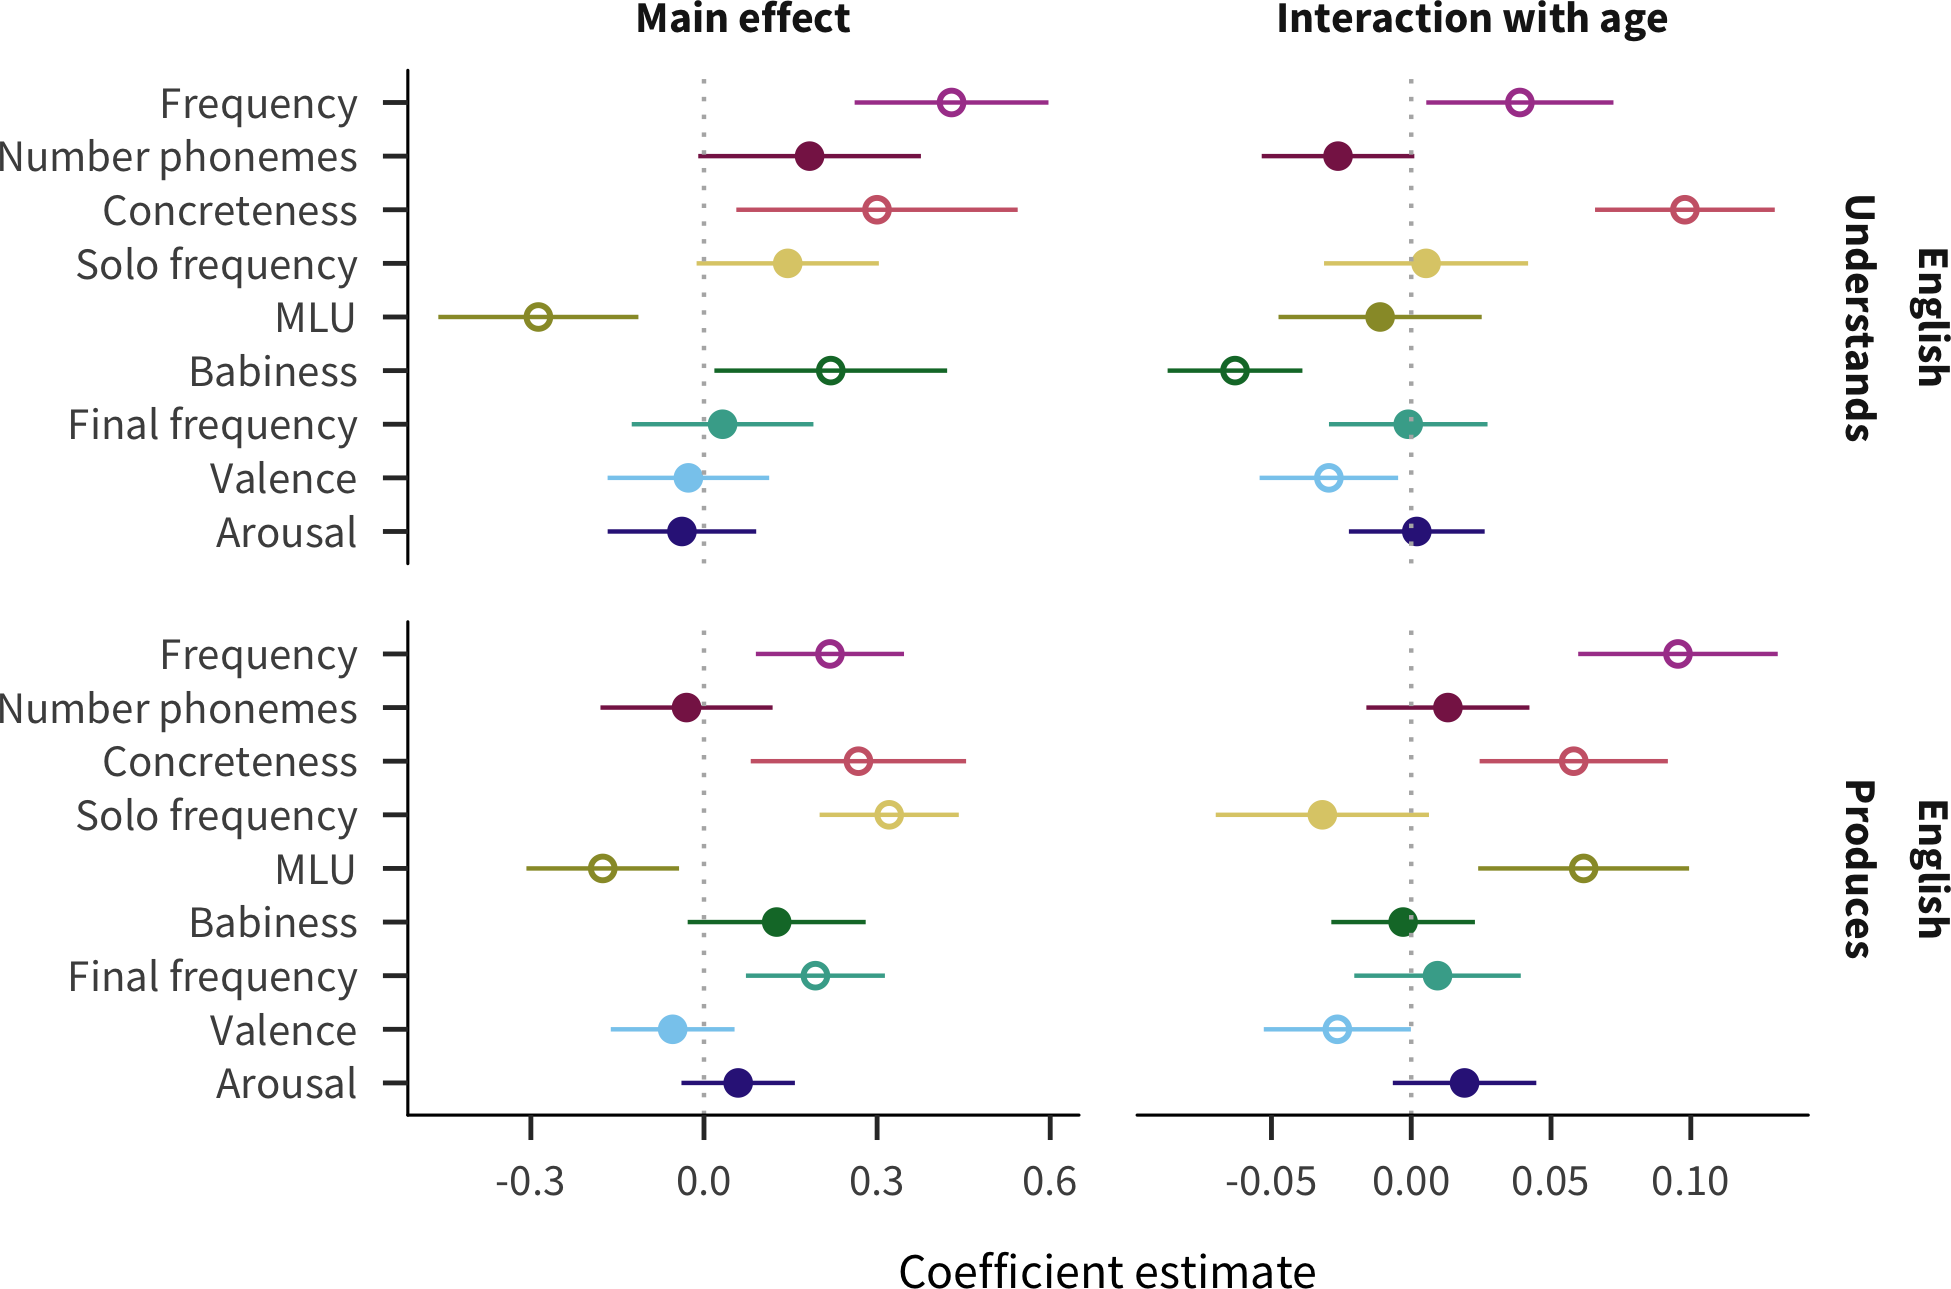
\includegraphics[width=\textwidth]{refcoefs-1}

}

\caption{Estimates of coefficients in predicting words' developmental trajectories for English comprehension and production data. Larger coefficient values indicate a greater effect of the predictor on acquisition: positive main effects indicate that words with higher values of the predictor tend to be understood by more children, while negative main effects indicate that words with lower values of the predictor tend to be understood by more children; positive age interactions indicate that the predictor's effect increases with age, while negative age interactions indicate the predictor's effect decreases with age. Error bars indicates 95\% confidence intervals; filled in points indicate coefficients for which $p < 0.05$.}\label{fig:refcoefs}
\end{figure}

\begin{figure}

{\centering 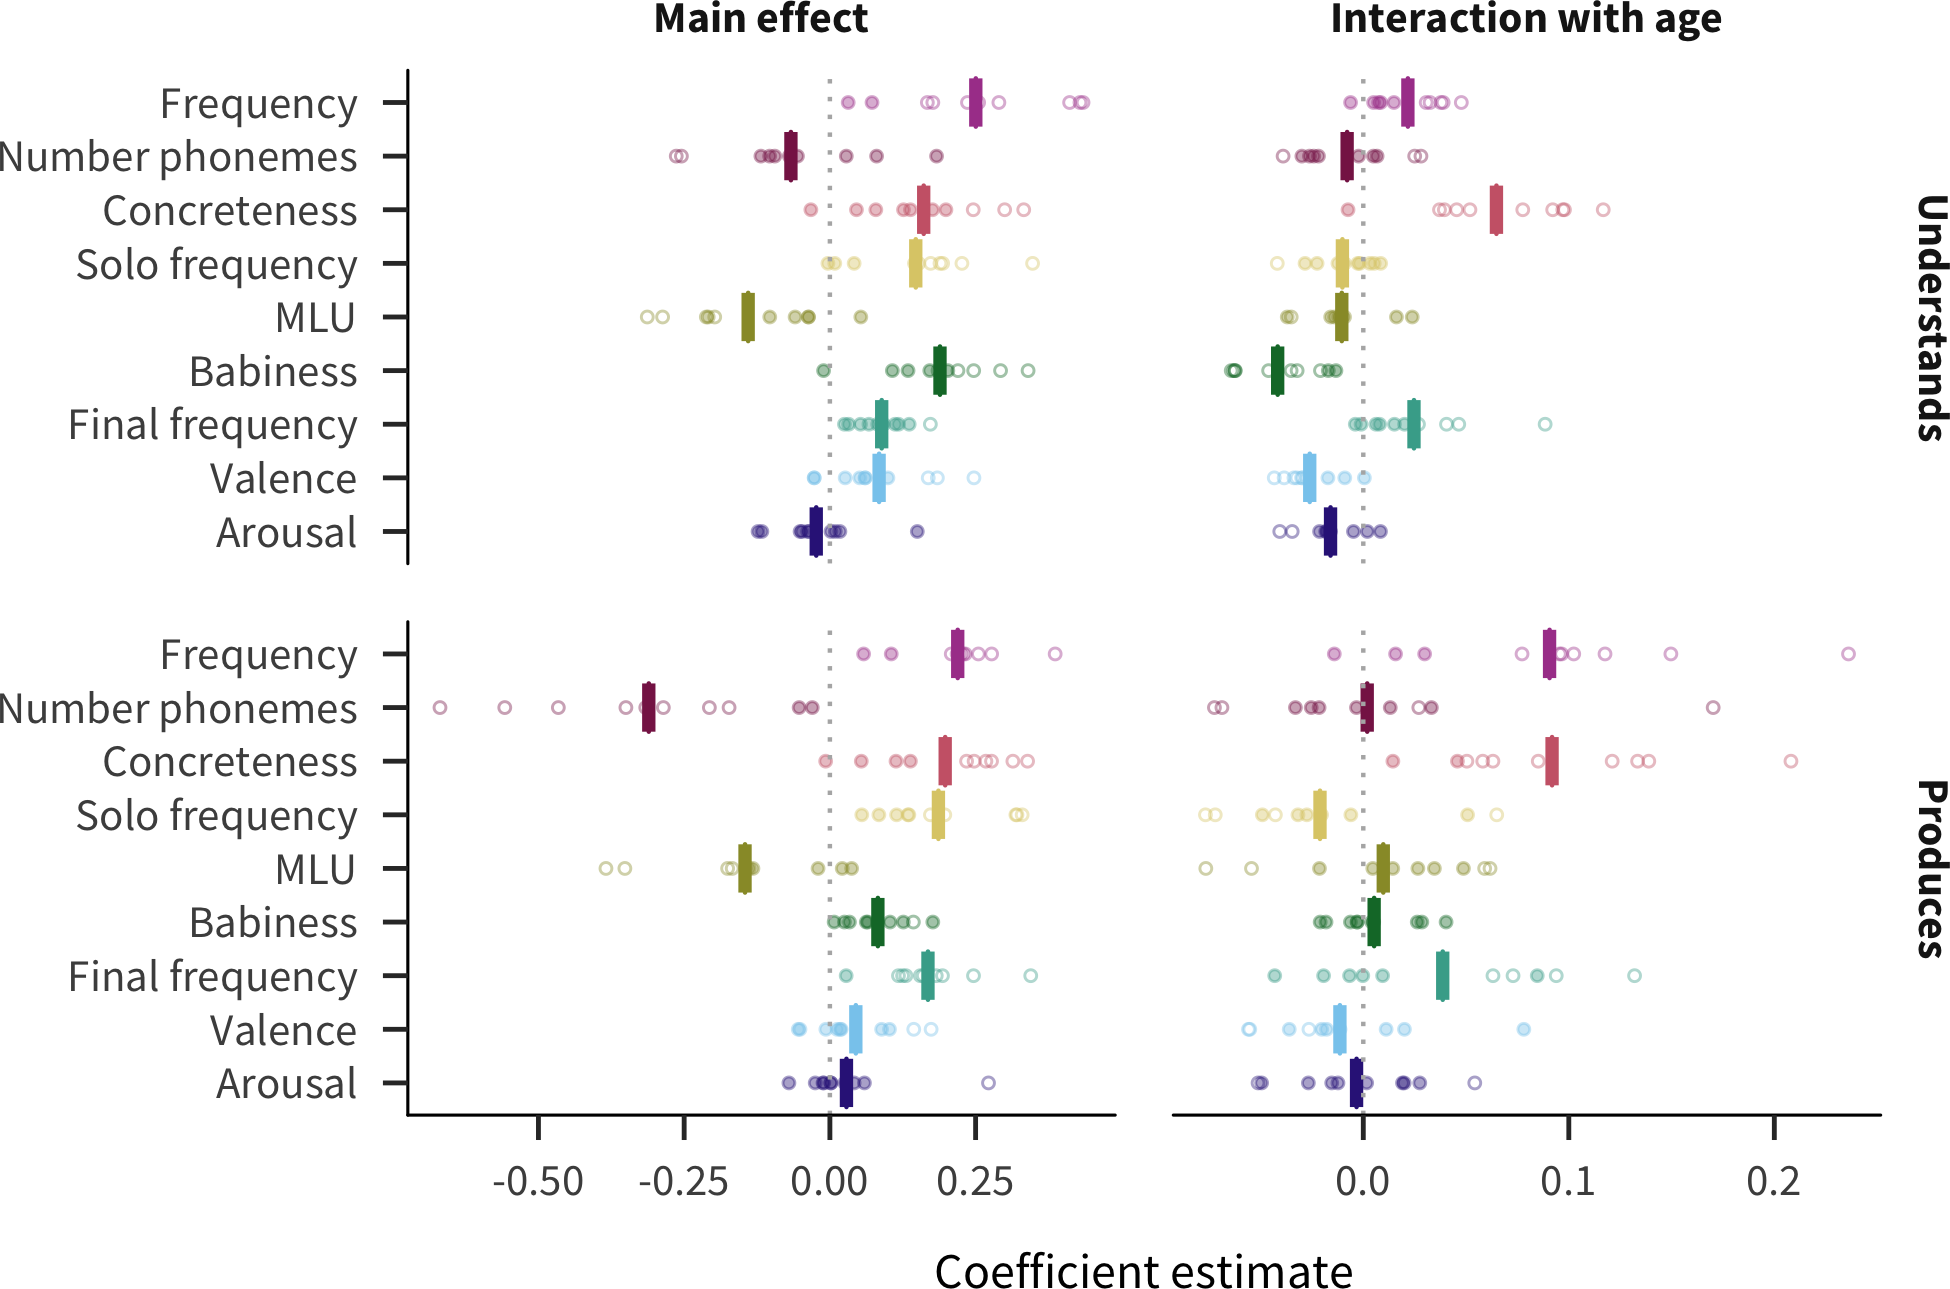
\includegraphics[width=\textwidth]{langcoefs-1}

}

\caption{Estimates of coefficients in predicting words' developmental trajectories for all languages and measures. Each point represents a predictor's coefficient in one language, with the bar showing the mean across languages. Filled in points indicate coefficients for which $p < 0.05$.}\label{fig:langcoefs}
\end{figure}

\subsubsection{English predictor effects}

To illustrate the structure of our analysis, we first describe the
results for English data, shown in Figure~\ref{fig:refcoefs} as the main
effect and age interaction coefficient estimates and 95\% confidence
intervals, for comprehension and production. For main effects, words are
more likely to be known by more children if they are higher in frequency
or concreteness, as well as in babiness for comprehension and in
sentence-final frequency or sole-constituent frequency for production.
In contrast, words that appear in shorter sentences (MLU) are more
likely to be reported as understood or produced. For age interactions,
while most predictors have consistent effects over age, words that are
higher in frequency or concreteness are more likely to be known more by
older children, while words that are higher in valence have a greater
effect on acquisition in younger children, with an additional negative
interaction with babiness in comprehension and positive interaction with
MLU in production.

\subsubsection{Cross-linguistic predictor effects}

Figure~\ref{fig:langcoefs} shows the coefficient estimate for each
predictor in each language and measure (for additional visualizations of
the coefficients, see Figures~SI.7, SI.8, and SI.9). We find that
frequency is the strongest predictor of acquisition (mean across
languages and measures \(\bar{\beta} = 0.23\)). Other relatively strong
overall predictors include concreteness (\(\bar{\beta} = 0.18\)), solo
frequency (\(\bar{\beta} = 0.17\)), MLU (\(\bar{\beta} = -0.14\)), and
final frequency (\(\bar{\beta} = 0.13\)). Number of phonemes is
comparatively large for production (\(\bar{\beta} = -0.31\)) but not
comprehension (\(\bar{\beta} = -0.07\)); conversely, babiness is
comparatively large for comprehension (\(\bar{\beta} = 0.19\)) but not
production (\(\bar{\beta} = 0.08\)). Finally, valence
(\(\bar{\beta} = 0.06\)) and arousal (\(\bar{\beta} = 0.003\)) have much
smaller effects.

Given the emphasis on frequency effects in the literature
\citep{ambridge2015}, one might have expected frequency to dominate, but
several other predictors are also quite strong. In addition, some
factors previously argued to be important for word learning, namely
valence and arousal \citep{moors2013}, appear to have limited relevance
when compared to other factors. These results provide a strong argument
for our approach of including multiple predictors and languages in our
analysis.

\begin{figure}

{\centering 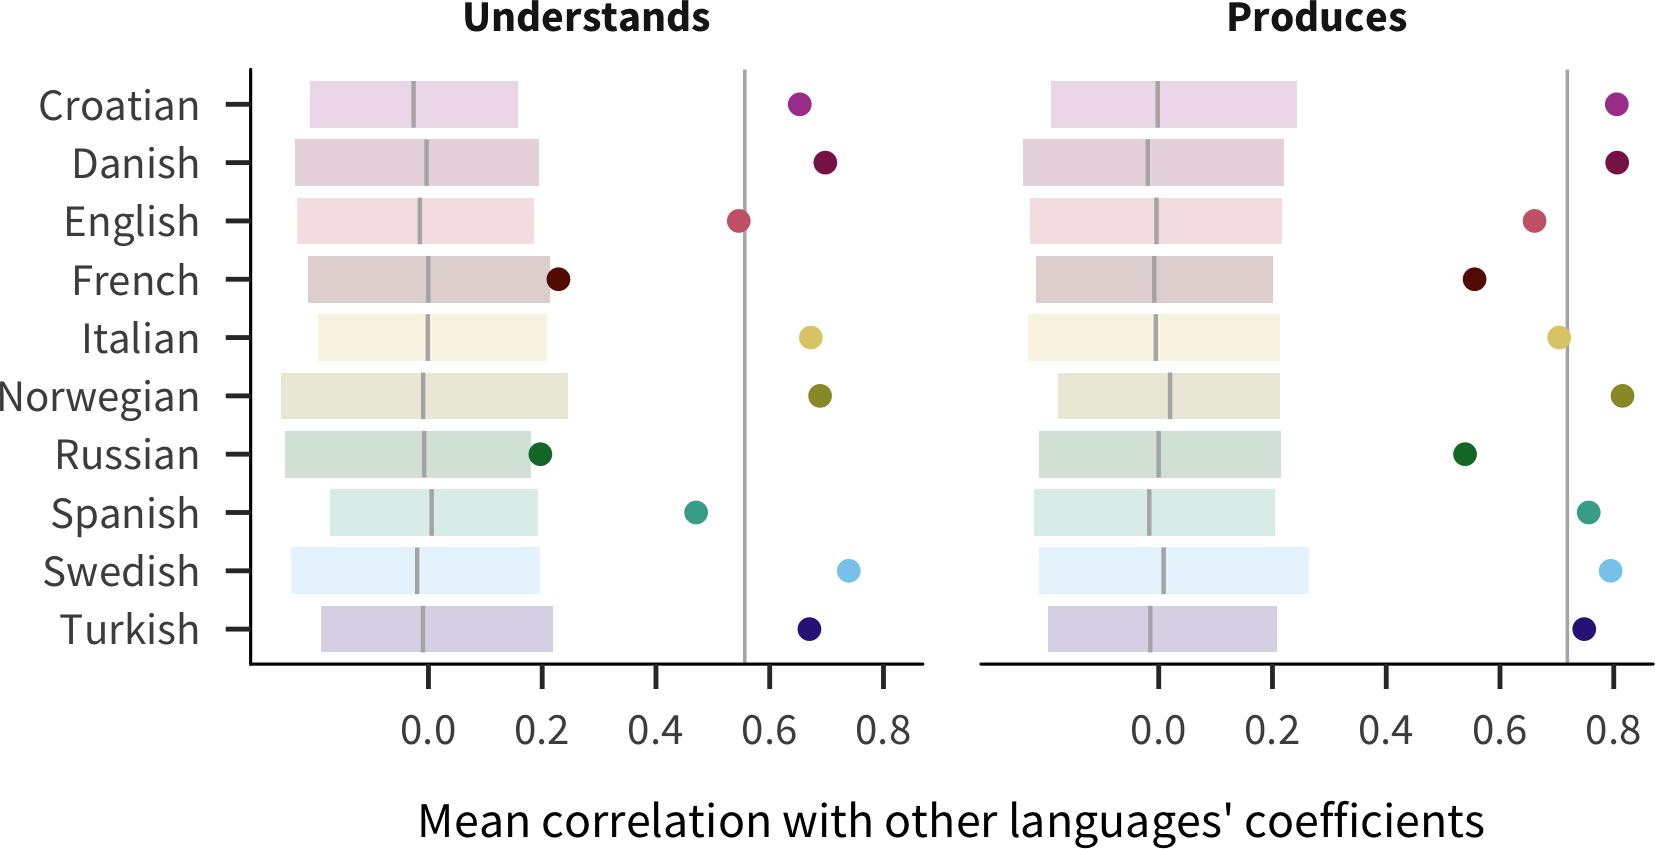
\includegraphics[width=\textwidth]{consistency-1}

}

\caption{Correlations of coefficient estimates between languages. Each point represents the mean of one language's coefficients' correlation with each other language's coefficients, with the vertical line indicating the overall mean across languages. The shaded region and line show a bootstrapped 95\% confidence interval of a randomized baseline where predictor coefficients are shuffled within language.}\label{fig:consistency}
\end{figure}

\begin{figure}

{\centering 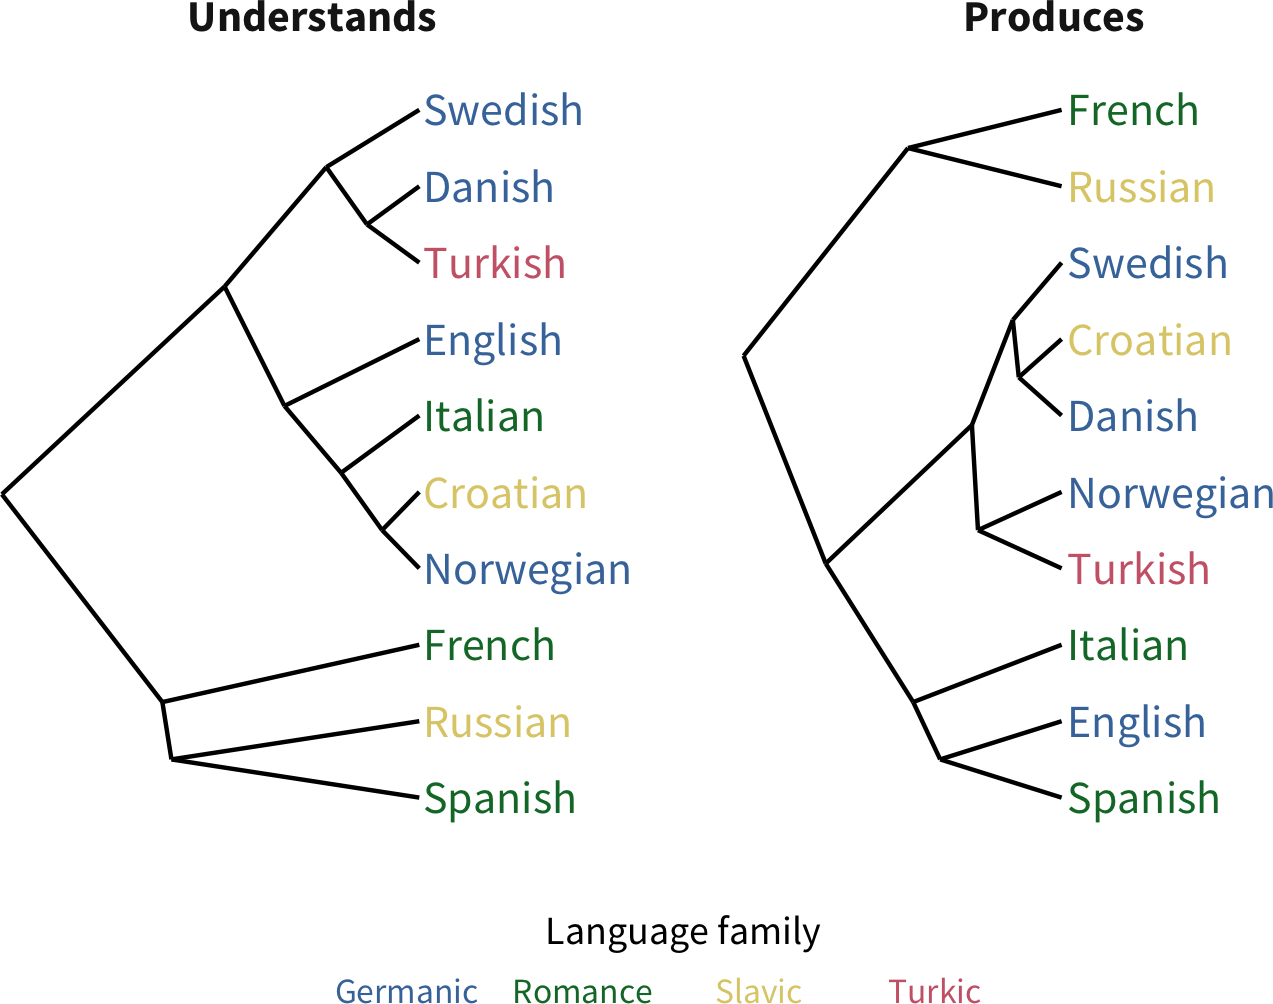
\includegraphics[width=0.7\linewidth]{clustering-1}

}

\caption{Dendrograms of the similarity structure among languages' coefficients.}\label{fig:clustering}
\end{figure}

\begin{figure}

{\centering 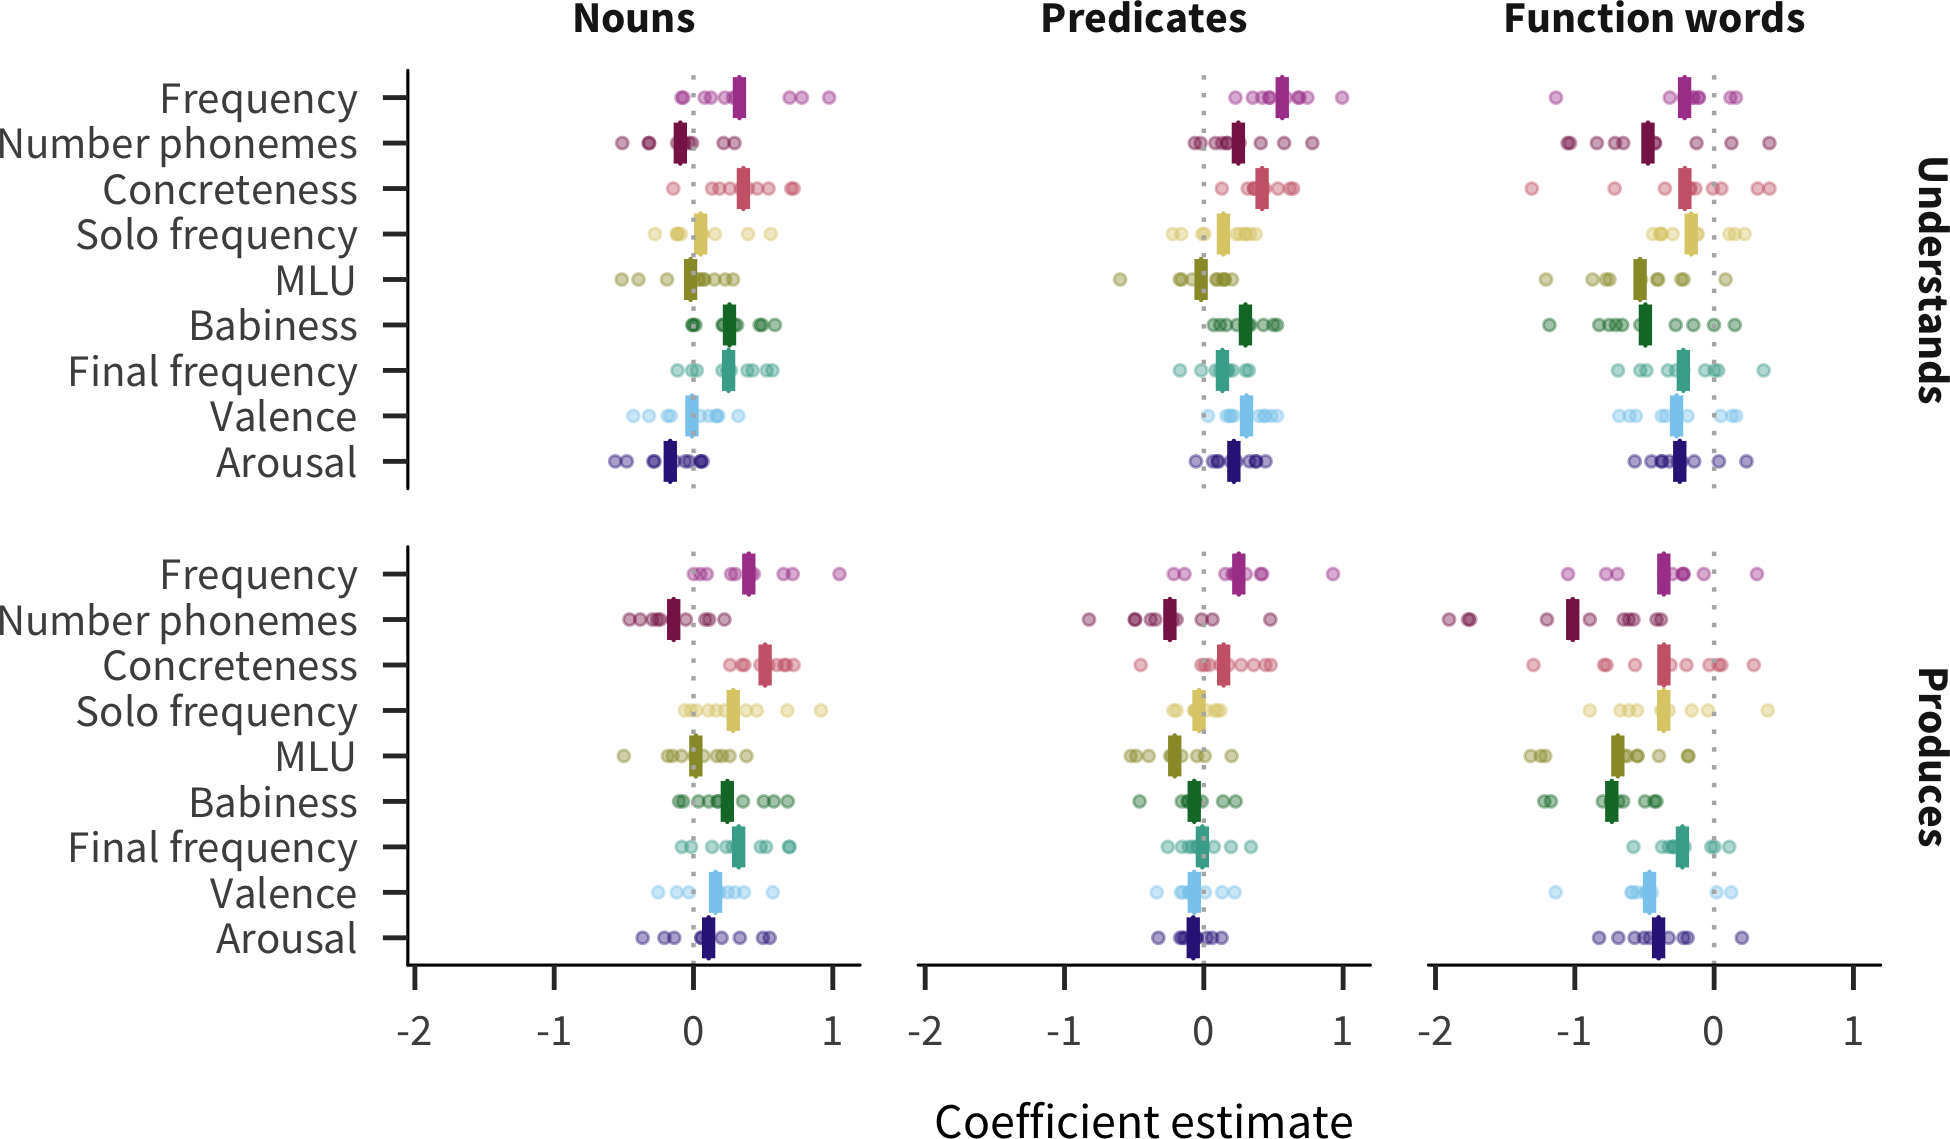
\includegraphics[width=\textwidth]{lexcatcoefs-1}

}

\caption{Estimates of effect in predicting words' developmental trajectories for each language, measure, and lexical category (main effect of predictor + main effect of lexical category + interaction between predictor and lexical category). Each point represents a predictor's effect in one language, with the bar showing the mean across languages.}\label{fig:lexcatcoefs}
\end{figure}

\subsubsection{Consistency}

Apart from valence and arousal, all other predictors have the same the
direction of effect in all or almost all languages and measures (at
least 17 of the 20). Thus, across languages, words are likely to be
understood and produced by more children if they are more frequent,
shorter, more concrete, more frequently the only word in an utterance,
more associated with babies, more frequently the final word in an
utterance, and appear in shorter utterances.

Additionally, there is considerable consistency in the magnitudes of
predictors across languages. A priori it could have been the case that
different languages have wildly different effects of various factors
(due to linguistic or cultural differences), but this pattern is not
what we observe. Instead, there is more consistency in the correlations
between coefficients across languages than would be expected by chance.
As shown in Figure~\ref{fig:consistency}, each language's mean pairwise
correlation with other languages' coefficients (i.e., the correlation of
coefficients for English with coefficients for Russian, for Spanish, and
so on) is outside of bootstrapped estimates in a randomized baseline
created by shuffling predictor coefficients within language. The
pairwise correlations are more consistent for production (mean 0.72)
than for comprehension (mean 0.56), in which French and Russian effects
are more idiosyncratic.

\subsubsection{Variability}

While some particular coefficients differ substantially from the trend
across languages (e.g., the effect of frequency for comprehension in
Spanish is near 0), these individual datapoints are difficult to
interpret. Many unmeasurable factors could potentially account for these
differences: Spanish frequency estimates could be less accurate due to
corpus sparsity or idiosyncrasy, the samples of children in the Spanish
CDI or CHILDES data could differ more demographically, or
Spanish-learning children could in fact rely less on frequency. Rather
than attempting to interpret individual coefficients, we instead ask how
the patterns of difference among languages reflect systematic
substructure in the variability of the effects.

To examine the substructure of predictor variability, we used
hierarchical clustering analysis to find the similarity structure among
the pairwise correlations between languages' predictors. The resulting
dendrograms are shown in Figure~\ref{fig:clustering}, which broadly
reflect language typology, especially for production data. This result
suggests that some language-to-language similarity is captured by the
profile of coefficient magnitudes our analysis returns.

\subsubsection{Comprehension vs.~production}

As mentioned above, word length is the one predictor of acquisition that
varied substantially between measures: it is far more predictive for
production than comprehension. Thus, as measured here, length seems to
reflect effects of production constraints (i.e., how difficult a word is
to say) rather than comprehension constraints (i.e., how difficult it is
to store or access). This result may explain why the hierarchical
clustering analysis above appears more similar to linguistic typology in
production than comprehension, that is, the role of production
difficulty may be more similar for more typologically-related languages.
Another possibility is that since the measures are confounded with age
(comprehension is only measured for younger children), word length may
play a larger role later in acquisition. Similarly, the stronger effect
of babiness in comprehension over production could be due to its larger
prominence earlier in development.

\subsubsection{Developmental change}

For both comprehension and production, positive age interactions can be
seen in at least 9 out of 10 languages for concreteness and frequency.
Conversely, there are negative age interactions for babiness and valence
for comprehension in at least 9 out of 10 languages. This suggests that
concreteness and frequency facilitate learning more so later in
development, while babiness and valence facilitate learning earlier in
development. This result is consistent with the speculation above that
the babiness predictor captures meanings that have special salience to
very young infants.

\subsubsection{Lexical categories}

Previous work suggests that predictors' relationship with age of
acquisition differs among lexical categories \citep{goodman2008}. We
investigate these differences by including lexical category interaction
terms in our model. Figure~\ref{fig:lexcatcoefs} shows the resulting
effects for each lexical category, combining the main effect of a given
predictor with the main effect of the lexical category and the
interaction between that predictor and that lexical category (see also
Figures~SI.10 and SI.11).

Across languages, the strongest predictors of acquisition for both nouns
and predicates are concreteness (nouns \(\bar{\beta} = 0.44\);
predicates \(\bar{\beta} = 0.28\)) and frequency (nouns
\(\bar{\beta} = 0.36\); predicates \(\bar{\beta} = 0.41\)). Thus content
words are most likely to be known by more children if they are more
frequent or more concrete. Conversely, function words are most
influenced by number of phonemes (\(\bar{\beta} = -0.74\)), babiness
(\(\bar{\beta} = -0.61\)), and MLU (\(\bar{\beta} = -0.61\)), meaning
that function words are most likely to be known by more children if they
are shorter, less associated with babies, or appear in shorter
sentences. These patterns are supportive of the hypothesis that
different word classes are learned in different ways, or at least that
the bottleneck on learning tends to be different, leading to different
information sources being more or less important across categories.

Additionally, the mean pairwise correlation of coefficients between
languages is much larger for nouns (0.68) and predicates (0.54) than for
function words (0.29). The higher between-language variability for
function words suggests the learning processes differ substantially more
across languages for function words than they do for content words (see
Figure~SI.12).

\section{Discussion}

What makes words easier or harder for young children to learn? Previous
experimental work has largely addressed this question using small-scale
lab studies. While such experiments can identify sources of variation,
they typically do not allow for different sources to be compared
directly. In contrast, observational studies allow the effects of
individual factors to be measured across ages and lexical categories
(e.g., \citealp{goodman2008,hills2009,swingley2017}), but are limited in
the size and scope of the datasets and languages that can be directly
compared. The current analyses take advantage of recent innovative
approaches via Wordbank, a large, cross-linguistic dataset of parent
report instruments. By compiling data regarding early lexical
development across 10 languages and examining patterns of acquisition in
relation to 9 predictors, our work expands the scope of these studies
dramatically, leading to several new findings.

First, we found consistency in the patterning of predictors across
languages at a level substantially greater than the predictions of a
chance model. This consistency supports the idea that differences in
culture or language structure do not lead to fundamentally different
acquisition strategies, at least at the level of detail we were able to
examine. Instead, they are likely produced by processes that are similar
across populations and languages. Such processes could include learning
mechanisms or biases internal to children, or interactional dynamics
between children or caregivers. We believe these consistencies should be
an important topic for future investigation.

Second, predictors varied substantially in their weights across lexical
categories. Frequent, concrete nouns were learned earlier, consistent
with theories that emphasize the importance of early referential speech
(e.g., \citealp{baldwin1995}). For predicates, concreteness was somewhat
less important and frequency some more important. And for function
words, length and MLU was more predictive, perhaps because it is easiest
to decode the meanings of function words that are used in short
sentences (or because such words have meanings that are easiest to
decode). Overall, these findings are consistent with some predictions of
both division of dominance theory, which highlights the role of
conceptual structure in noun acquisition \citep{gentner2001}, and
syntactic bootstrapping theory, which emphasizes linguistic structure
over conceptual complexity in the acquisition of lexical categories
other than nouns \citep{snedeker2007}. More generally, our methods here
provide a way forward for testing the predictions of these theories
across languages and at the level of the entire lexicon rather than
individual words.

In addition to these new insights, several findings emerged that confirm
and expand previous reports. Environmental frequency was an important
predictor of learning, with more frequently-heard words learned earlier
\citep{goodman2008,swingley2017}. Predictors also changed in relative
importance across development. For example, certain words whose meanings
were more strongly associated with babies appeared to be learned early
for children across the languages in our sample (as in
\citealp{tardif2008}). Finally, word length showed a dissociation
between comprehension and production, suggesting that challenges in
production do not carry over to comprehension (at least in parent-report
data).

Despite its larger scope, our work shares a number of important
limitations with previous studies. First and foremost, our approach is
to predict one set of individuals with data about the experience of a
completely different set and conceptual ratings gathered from yet
others. In contrast to dense-data analyses \citep{roy2015}, this
approach fundamentally limits the amount of variability we will be able
to capture. Second, the granularity of the predictors that can be
extracted from corpus data and applied to every word is necessarily
quite coarse. Ideally, predictors could be targeted more specifically at
particular theoretical constructs of interest (e.g., the patterns of use
for specific predicates). Third, our analyses are conducted within
language, so to the extent that the predictors can have differing ranges
in different languages, cross-linguistic patterns in predictor effects
could be obscured.

Finally, our data are observations gleaned from parent report. CDI
instruments are both reliable and valid, and the cross-linguistic
adaptations we used contain the original researchers' best attempts to
create culturally-appropriate word lists. Nevertheless, this
observational design introduces many sources of uncertainty and bias.
First, the open data format of Wordbank reflects the sampling and
administration methods of many groups around the world; these introduce
many unknown biases that we cannot control (though they would likely not
contribute to observed consistencies). Second, language and culture
co-vary completely in our sample and so variability that we observe
cannot be attributed to one or the other. Finally, some observed
consistencies could arise from consistency in parental reporting biases.
For example, across languages, parents might be generally biased to
under-report comprehension of function words. Despite the quantity of
data analyzed here, our conclusions will require further testing through
converging evidence from both laboratory experiments and direct
observation.

In sum, by examining predictors of early word learning across languages,
we identified substantial cross-linguistic consistency in the factors
contributing to the ease or difficulty of learning individual words.
This suggests that common learning mechanisms and/or environmental
supports for learning are shared across all of these languages. These
findings also testify to the importance of building open, shared
resources in the study of child language learning -- without the efforts
of many research groups across many language communities, such studies
would be impossible. Additionally, we hope that our work here provides a
baseline for the building of future predictive models that allow
theories of language learning to be tested at scale.

%%% End of Article


\acknowledgments
Thank you to the labs and individuals who contributed data to Wordbank
and to NSF BCS \#1528526 for support.

\authorcontributions
M.B. and D.Y. conducted data processing and analysis, with supervision
from V.A.M. and M.C.F.; all authors contributed to writing the paper.

\bibliography{aoapred}

\end{document}
